\chapter{Integrace do výuky a využití}
Již v~průběhu psaní této práce jsou materiály z~výukové sady využívány vyučujícími a studenty naší školy, možná i jiných středních průmyslových škol.
Kromě nich je využívají i~někteří vysokoškoláci.

\section{Sledovanost v~číslech}
Ke dni 24. 5. 2021 se celkový počet zhlédnutí všech veřejných videí pohybuje okolo 2,6 tisíce (počet zhlédnutí dle YT analytics je 2662).
Obecně nejsledovanějším videem je návod na instalaci SolidWorks SDK 2020/2021 se 746 zhlédnutími, které bylo distribuováno primárně mezi studenty naší školy (video je neveřejné a dostupné pouze pomocí odkazu uvedeného v~příloze \ref{released-videos}).
Za ním se nachází video zaměřené na modelování ozubeného kola s~přímým ozubením s~579 zhlédnutími.

Návštěvnost webového portálu P3D se aktuálně pohybuje v~řádu stovek.
Ke dni 24. 5. 2021 zaznamenal tento web přibližně 800 návštěvníků.

\begin{figure}
    \centering
    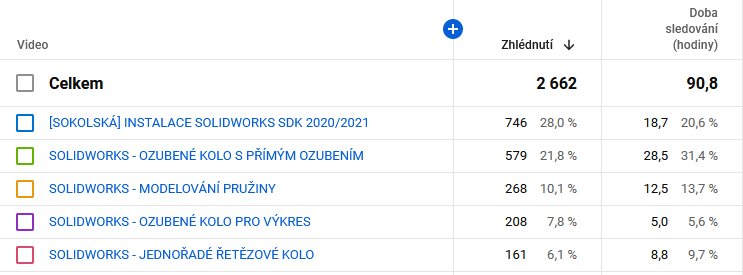
\includegraphics[width=0.7\textwidth]{img/020/yt-analytics-24-05-21.png}
    \caption{Snímek analytiky YouTube ze dne 24. 5. 2021}
    \label{fig:yt-analytics}
\end{figure}

\section{Distanční výuka}
Výuková videa našla při distanční výuce podstatné využití.
Videokonferenční programy nezaručují dostatečně vysokou kvalitu přenosu obrazu ani zvuku, kvůli čemuž by musel vyučující ukázku postupu při výpadku na straně studentů často opakovat.
Učitelé na naší škole proto v~některých případech vlastní ukázky zcela nahrazují odkazováním na mnou vytvořená výuková videa a materiály, jelikož jsou schopny tyto ukázky plně zastoupit.
Sami studenti tyto materiály využívají při práci na svých projektech, jelikož kvůli absenci prezenční výuky nemají možnost pracovat v~hodinách za přítomnosti učitele a nemohou se na něj tedy obrátit s~žádostí o~pomoc.
Ti zvídavější z~nich se pomocí mých materiálů mohou učit nové postupy, ke kterým v~běžné výuce ještě nedošli.

\section{Využití materiálů v~prezenční výuce}
K~praktickému využití v~prezenční výuce bohužel z~důvodu celosvětové pandemie zatím nedošlo. 
I~přesto je jejich implementace do výuky strojírenské konstrukce plánovaná přinejmenším na naší škole.
Většina vyučujících je začne s~obnovením prezenční výuky využívat a v~příštím roce bych rád praktickou aplikaci svých materiálů dále rozšířil.

Vzhledem k~tomu, že jsou všechny materiály volně dostupné, jejich využití je proto možné i na jiných školách.
S~tím se pojí i velmi snadné začlenění do výuky.
Vyučující nemusí nic složitě hledat -- na webových stránkách snadno a rychle najde vytisknutelné materiály i výuková videa.
Textové materiály samozřejmě není nutné používat jen v~papírové podobě. Studentům je může snadno rozeslat ve formátu PDF, popřípadě může jen odkázat na webové stránky \href{https://www.p3dportal.cz}{www.p3dportal.cz}.

Způsobů využití mojí výukové sady v~prezenční výuce existuje celá řada.
Vyučující upřednostňující textovou formu mohou studentům vytisknout a rozdat materiály nebo jim je snadno rozeslat.
Pokud je v~učebně k~dispozici projektor, mohou promítat výuková videa, případně nechat studenty, aby je sledovali samostatně na svých počítačích.
Další možností je kombinované využití výukových videí a tištěných materiálů, kdy vyučující pomocí projektoru nechá studenty zhlédnout video, následně jim rozdá vytisknuté materiály a nechá je vypracovat úkoly a otázky, které jsou v~nich obsaženy.
